\subsection{External Memory}

\subsubsection{Hard Disk Drives (HDD) - Magnetic Disks}

\begin{figure}[H]
    \centering
    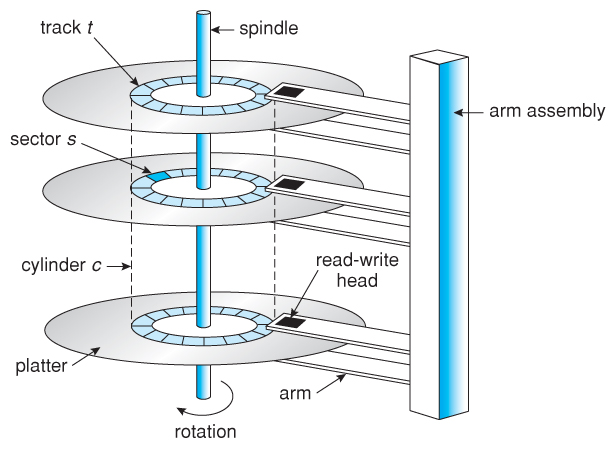
\includegraphics[width=0.58\textwidth]{chaps/memory/external-memory/hdd-layout.jpg}
    \caption{Disk Data Layout}
\end{figure}

\textbf{Terminologies about the HDD layout and components}:
\begin{itemize}
    \item \textbf{Platter}: Magnetically coated disks.
    \item \textbf{Track}: Concentric rings on a platter.
    \item \textbf{Sector}: A segment of a track, usually 512 bytes.
    \item \textbf{Cylinder}: Tracks of different platters that are under the read/write head
        at the same time.
\end{itemize}

\textbf{Formats of Tracks} -- Tracks contain sectors that hold data and other bits that
are useful for the disk controller. The example of a track format can be:
\begin{itemize}
    \item Each track contains 30 sectors of fixed-length 600 bytes, with 512 bytes for data
        and 88 bytes for control information.
    \item Each sector contains several fields: \begin{itemize}
        \item \textbf{Gap 1} (17 bytes): Used to separate sectors.
        \item \textbf{ID Field}: Contains Synch (1 byte), Track, Head, Sector \# (4 bytes),
            and CRC (2 bytes).
        \item \textbf{Gap 2} (41 bytes): Used to separate ID field and data field.
        \item \textbf{Data Field} (515 bytes): Contains 1 Synch byte, 512 bytes of data, and 2
            CRC bytes.
        \item \textbf{Gap 3} (40 bytes)
    \end{itemize}
\end{itemize}

\begin{wrapfigure}{l}{0.6\textwidth}
    \centering
    \begin{subfigure}{0.28\textwidth}
        \centering
        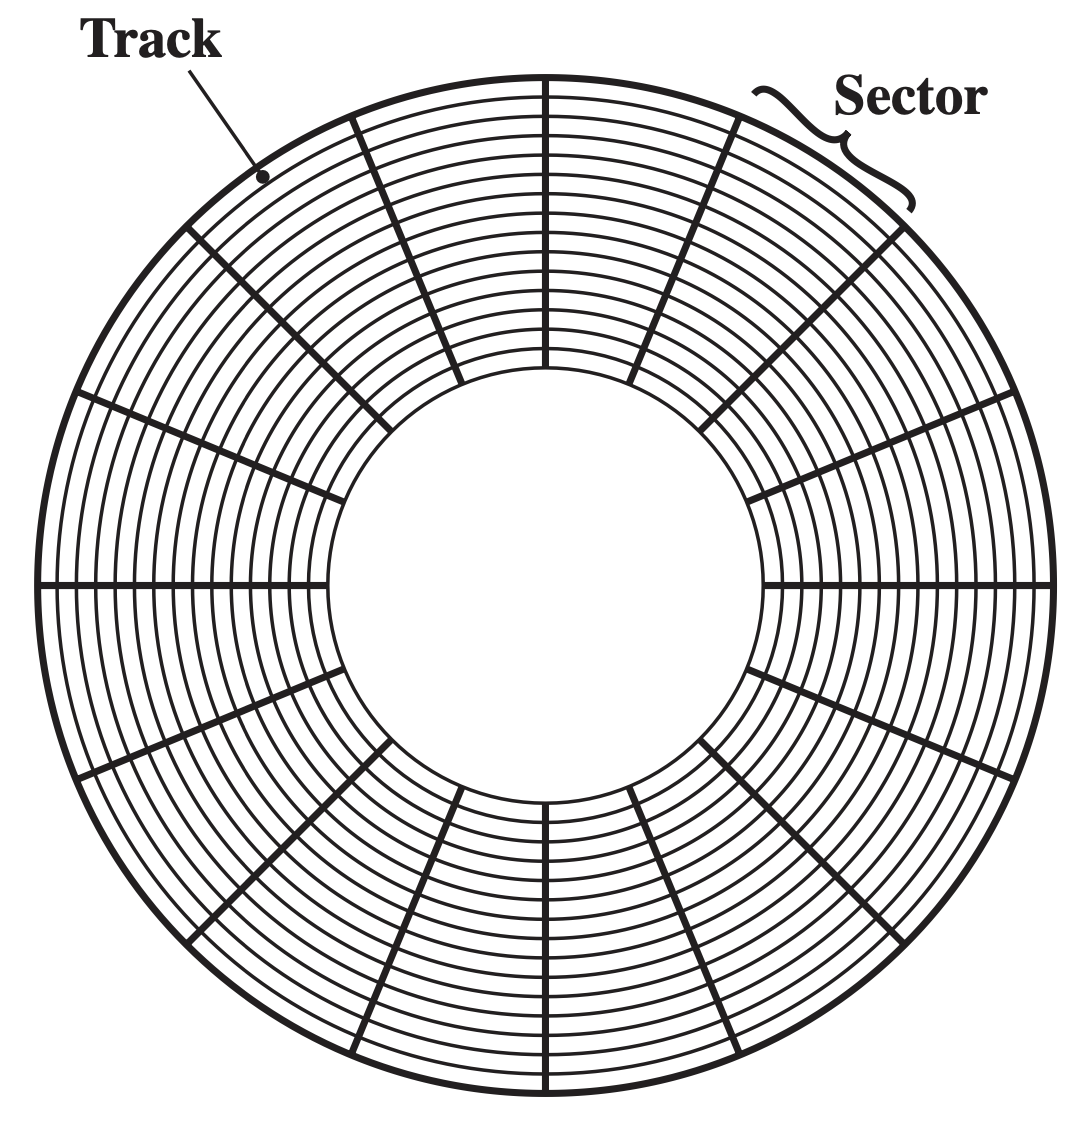
\includegraphics[width=\textwidth]{chaps/memory/external-memory/disk-layout-cav.png}
        \caption{CAV}
    \end{subfigure}
    \hfill
    \begin{subfigure}{0.28\textwidth}
        \centering
        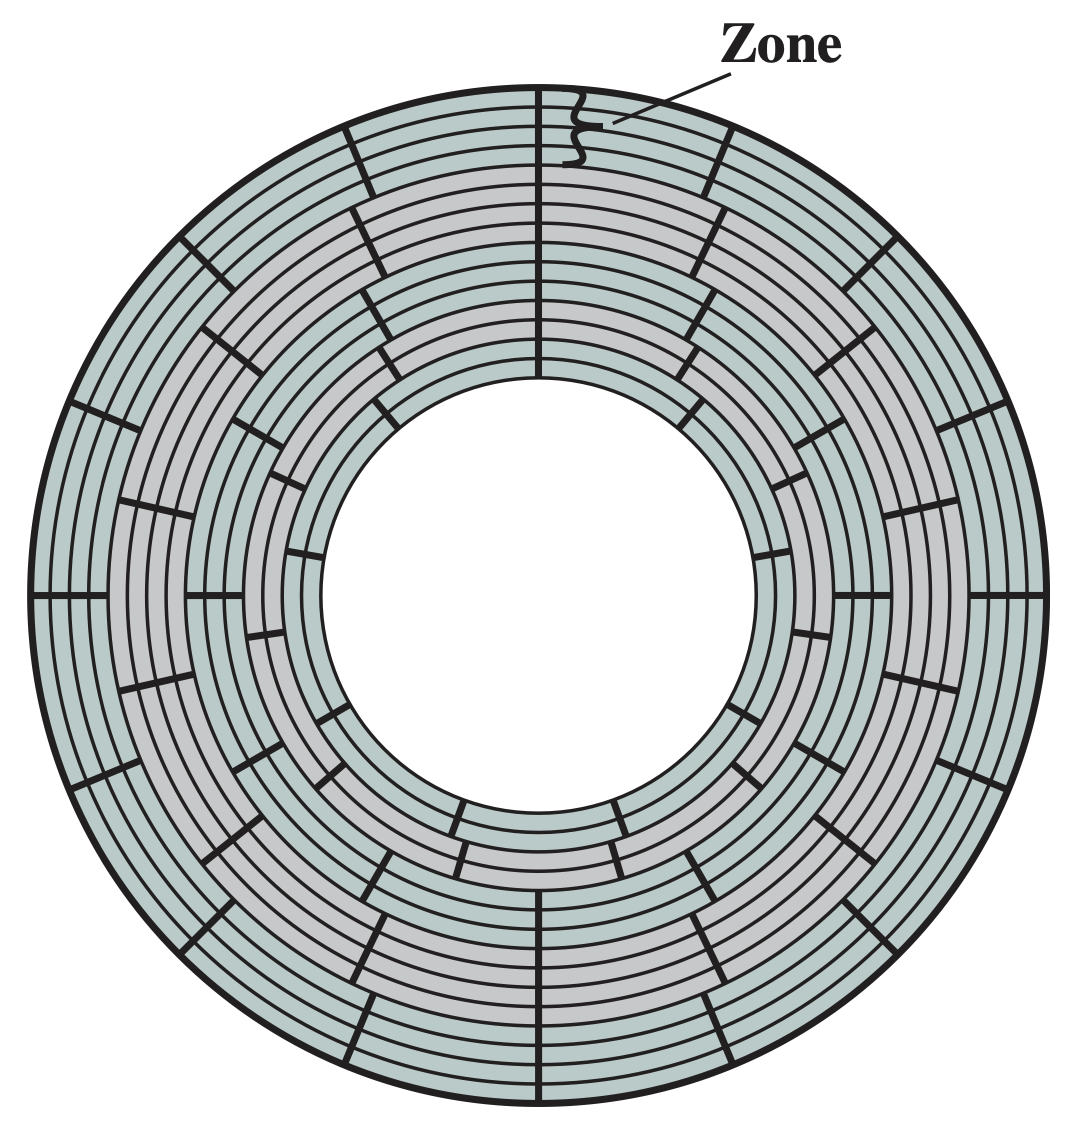
\includegraphics[width=\textwidth]{chaps/memory/external-memory/disk-layout-mzr.png}
        \caption{MZR}
    \end{subfigure}
    \caption{Disk Layout Methods}
\end{wrapfigure}

\textbf{Disk Layout Methods}:
\begin{itemize}
    \item \textbf{Constant Angular Velocity (CAV)}: Blocks of data can be directly addressed
        by track and sector. Read/write is easy. However, density of data decreases from the
        inner tracks to the outer tracks, which wastes space.
    \item \textbf{Multiple Zone Recording (MZR)}: Divides the disk into zones, with each zone
        having a different number of sectors per track. Note that the data density is not
        exactly the same, but only approximated to be the same. This allows maximised storage
        capacity.
\end{itemize}